

\title{Learning the blending spikes using sparse dictionaries}
\renewcommand{\thefootnote}{\fnsymbol{footnote}}

\author{Yangkang Chen\footnotemark[1], Shaohuan Zu\footnotemark[1], Wei Chen\footnotemark[2]\footnotemark[3], Mi Zhang\footnotemark[4],  and Zhe Guan\footnotemark[5]}
\ms{GJI-2020} 

\address{
\footnotemark[1]
School of Earth Sciences\\
Zhejiang University\\
Hangzhou, Zhejiang Province, China, 310027\\
yangkang.chen@zju.edu.cn \\
\footnotemark[2]Key Laboratory of Exploration Technology for Oil \\
and Gas Resources of Ministry of Education\\
Yangtze University\\
Daxue Road No.111\\
Caidian District, Wuhan, China, 430100\\
\footnotemark[3]Hubei Cooperative Innovation Center of Unconventional Oil and Gas\\
Daxue Road No.111\\
Caidian District, Wuhan, China, 430100\\
chenwei\_yangtze@126.com \\
\footnotemark[4]State Key Laboratory of Petroleum Resources and Prospecting \\
China University of Petroleum \\
Fuxue Road 18th\\
Beijing, China, 102200 \\
cupmi@sina.com \\
\footnotemark[5]
Applied Physics Program\\
Rice University\\
Houston, TX, USA\\
Zhe.Guan@rice.edu\\
}

\lefthead{Chen et al.}
\righthead{Learning the spikes}

\begin{abstract}
Deblending plays an important role in preparing \dlo{the }high-quality seismic data from modern blended simultaneous-source seismic acquisition. \dlo{The s}\wen{S}tate-of-the-art deblending\dlo{ method} is based on the \old{sparsity-constraint}\new{sparsity-constrained} iterative inversion. \dlo{The inversion}\wen{Inversion} based deblending\dlo{ method} assumes that the ambient noise level is low and the data misfit during iterative inversion accounts for the random ambient noise. The traditional method becomes problematic when the random ambient noise becomes extremely strong and the inversion iteratively fits the random noise instead of the signal and blending interference. We propose a \dlo{novel }constrained inversion model that takes the strong random noise into consideration and can achieve satisfactory result even when strong random noise exists. The principle of \dlo{the}\wen{this} new method is that we use sparse dictionaries to learn the blending spikes and thus the learned dictionary atoms are able to distinguish between blending spikes and random noise. The separated signal and blending spikes can then be better fitted by the iterative inversion framework. \dlo{A set of synthetic}\wen{Synthetic} and field data examples are used to demonstrate the performance of the new approach. \\
\textbf{Keywords}\\
Geophysical methods, Time series analysis, Image processing, Seismology
\end{abstract}

%\section{Keywords}
%key1,key2,key3

\DeclareRobustCommand{\dlo}[1]{}
\DeclareRobustCommand{\wen}[1]{#1}


\section{Introduction}
Simultaneous-source acquisition technique is a breakthrough in modern seismic data acquisition \cite[]{beasleycj2008,berkhout2008,abma2009,beasley2012,berkhout2012,wapenaark2012,qushan2015,abma2015,shaohuan2017jag,asgedom2017rough,zhang2017improving,kim2017efficient,shaohuan2017jag,wang2017building,wujuan2018jse1,amundsen2017multi}. It removes the limit of large temporal/spatial interval between adjacent shots or consecutive shots by allowing multiple sources to be fired simultaneously. The technique can not only improve the quality of recorded seismic data by increasing the spatial sampling rate but also increase the acquisition efficiency by decreasing the shot interval between two consecutive shots. However, the simultaneous-source acquisition will cause strong crosstalk interference in the recorded data, which makes the subsequent seismic data processing challenging. Because of the benefits of the revolutionary acquisition concept and the challenges involved in the processing and imaging framework, the technique has attracted much attention from both industry and academia \cite[]{mahdad2011,mahdad2012,panagiotis20122,arazthesis2012,qushan2014,sixuethesis2014,yanhui2014,sixue2015,halliday2015,benfengpocs,sixuethesis2014,sixue2015,yangkang2016irr5d,Robertsson2016Signal,andersson2017flawless,yatong2018gji,baimin2018jse2,yatong2018dbi,yatong2018jse}. 

The \dlo{blended }simultaneous-source seismic data can either be separated first and then be used for seismic imaging or be used directly for imaging. The former strategy is referred to as \dlo{the }deblending\dlo{ process} while the latter strategy is referred to as\dlo{ the} direct imaging\dlo{ method}. Deblending can provide a dataset that is similar to those datasets acquired from \dlo{the}\wen{a} traditional acquisition system, thus does not require the modification of the \wen{present} seismic imaging algorithms. However, due to its \dlo{dependency}\wen{dependence} on the pre-processing of massive blended data, it is more computationally expensive. The direct imaging method avoids the pre-processing step, but requires a carefully modified seismic imaging framework. A number of great breakthroughs have been made on direct imaging of simultaneous-source data recently \cite[]{verschuur2011,shuwei2016vscan,kui2016,kui20162,shaohuan2017,baimin2017jse1,yangkang2017lsrtm,wujuan2018cg1,baimin2018jse1,baimin2018cg,qingchen2018tgrs,qingchen2018gji,yangkang2019lsrtm}, thus in this paper we limit the discussion only on the deblending methods.


Among all the deblending methods, most are based on the spatial coherency of useful signals and incoherency of blending interference \cite[]{wujuan2019jse1}. To promote the coherency of useful signals, the seismic data should be sorted into the common receiver domain, common midpoint domain or common offset domain. In the ocean bottom node (OBN) seismic surveys, the seismic data is recorded in the common receiver domain, thus, it is straightforward to apply the deblending algorithms without domain transformation \cite[]{arazthesis2012}. \cite{kim2009} applied an offset-domain prediction and subtraction method to iteratively attenuate the blending spikes. The blending spikes refer to the blending noise. Because the blending noise is spatially discontinuous and has abnormal value, like spikes, we call the blending noise \old{as }blending spikes throughout the paper. \cite{yangkang20142} initially proposed a general iterative framework for iterative estimation and subtraction of blending spikes based on the shaping regularization method. In the shaping regularization framework, most iterative deblending methods can be understood in the same way except for a different constraint or assumption for the model.

A large group of deblending methods are based on the sparsity. \cite{akerberg2008} proposed an iterative deblending method based on the Radon transform. \cite{abma2009} used the Fourier transform to promote the sparsity of useful signals and developed an effective deblending method, which has now been widely applied in the industry. \cite{yangkang20142} used the seislet transform, which is assumed to be the sparest transform for seismic data, to promote the sparsity of useful signals and separate the crosstalk noise. \cite{yangkang2015dbortho} further extend the seislet constraint to a hybrid orthogonalization and seislet constraint to better separate the blended sources. \cite{shaohuan20161} used the curvelet transform as the sparse domain to separate the blended sources. They also pointed out that the traditional random dithering sequences are not optimal in practical deployment of the technique in the field and proposed a periodic shot scheduling sequence for blended acquisition. \cite{yaru20172} used the high-order sparse Radon transform to deal with the amplitude-variation-with-offset (AVO) phenomenon that is usually neglected in deblending frameworks. \cite{yatong2018seis} applied the seislet frame transform to filter out blending spikes in the presence of multiples. Because the multiples have different local slopes, the seislet frame transform\dlo{ instead of seislet transform} is used to sparsify multiples with different orders. In addition to the sparsity constraint \cite[]{mostafa2016geo,mostafa2016bssa}, the rank constraint is also used for the deblending purposes \cite[]{yaru2016dblend,zhangdong2016cseg,zhangdong2016seg,zhangdong2016eage,wujuan2018jge3,baimin2019jag}. \cite{jinkun2015} developed the iterative rank-reduction method for deblending simultaneous-source data, where the singular spectrum analysis (SSA) filter is applied as the shaping operator. \cite{yatong2017ieee} applied the structural rank-reduction method for attenuating the blending spikes, where the rank-one approximation filter is applied as the rank-reduction operator. Similar to the sparsity and rank constraints, the coherency constraint was proposed by \cite{shaohuan2017gji} to deal with the complicated situations where data structure is complex and the number of simultaneous sources is large.

%\cite{yatong2018seis} propose
Another mainstream method for deblending is not based on the coherency difference between useful signals and blending spikes. According to the local slope difference between signals and noise, \cite{hampson2008} applied a dip filter to remove the blending interference in common shot gathers. \cite{sixue2015} analyzed the disadvantage of the receiver-domain deblending methods and proposed a shot-domain deblending method based on the shot repetition concept. They argue that data in the receiver domain are usually under-sampled and is \dlo{easier}\wen{more prone} to cause the aliasing problem than the data in shot domain. \cite{shuwei20163} developed an iterative seislet frame thresholding method to separate simultaneous-source data in the shot domain. The seislet frame can compress the \dlo{master shot and interference shot}\wen{signal and interference} according to their individual slope maps, which can be calculated directly from the blended data in the shot domain. \cite{shaohuan2017} proposed a least-squares method for separating the \dlo{master shot and interferening shot}\wen{signal and interference} in the shot domain. The crux of the least-squares method is constructing two convolutional filters to set up a least-squares estimation problem. The convolutional filters are constructed based on the plane-wave approximation of wave equation.   

In this paper, we address the problem of strong ambient noise in iterative inversion based deblending framework. It is known that the iterative inversion method is based on small random noise level, i.e., small and negligible data misfit. The source-separation inversion uses least-squares method to adjust the data misfit caused by random ambient noise. When the noise level is high, the least-squares method will try to fit the noise component instead of the blended signal components. To unravel the challenge in deblending when strong random noise exists, we propose a method to distinguish the blended signal components and the random noise by designing a dictionary that can best represent the waveform structure of both signal and blending spikes. By learning the structure of \wen{the} blending spikes, we are able to separate the blending spikes from random noise and thus make the iterative inversion robust. We first briefly introduce the sparse-inversion framework for the deblending problem and then introduce the dictionary learning constrained deblending framework in detail. To illustrate the philosophy of the presented method, we use \dlo{extensive }numerical examples to demonstrate the performance of the new method.

The concept of sparse dictionary learning \cite[]{mairal2009online}, originated from image processing field,  and is not new in geophysics. Many applications of the sparse dictionary learning algorithm have been investigated in the geophysics literature \cite[]{jianwei20142,yangkang2016dsd,amir2017geo,amir2017}. However, most of the applications are about representing spatially coherent reflection seismic events in a sparse way so that the spatially incoherent components can be easily separated during the sparse learning process. The application of the sparse dictionary learning algorithm here is somewhat contradicting with the mainstream studies, i.e., we want to represent the blending spikes using the sparse dictionary learning method. The benefit of the sparse representation of blending spikes is that we can relieve the influence of the random noise to iterative deblending of simultaneous-source data by separating the random noise based on the hybrid-sparsity constrained model for deblending. This type of application of dictionary learning is unusual not only in the deblending literature, but also in the whole seismic data processing community. Blending spikes, due to its spatial incoherency property, are thought to be excluded from being \old{learned into}\new{learned by} the dictionary atoms \cite[]{yanhui2014,yanhui2016}. However, in this paper, we have shown using extensive examples that the blending spikes can be learned via a normal sparse dictionary learning algorithm for being separated from random noise and their features can be well captured by the dictionary atoms. This phenomenon can be attributed to the fact that although the blending spikes are not spatially coherent, they are temporally coherent. The blending spikes share the same properties with the useful primary signals when viewed in the time \old{direction}\new{dimension}. We infer that the temporal coherency property of the blending spikes \old{make}\new{makes} them easy to be learned by a typical sparse dictionary learning algorithm, e.g., the K-SVD method \cite[]{aksvd2008}. From the experiments and results shown in this paper, we are questioning the possibility of using a sparse dictionary learning based algorithm to separate the blending interference from the primary reflection signals, e.g., the work from \cite{yanhui2014}. If we do want to apply the sparse dictionary learning method to separate the blending spikes only, we need to adjust the typical dictionary learning algorithm so that the blending spikes cannot be taken into consideration when constructing the dictionary atoms. For example, constraining the dictionary atoms not to contain spikes may be a potential solution.

\section{Method}
\subsection{Iterative deblending as an optimization problem}
Regularized iterative deblending is equivalent to solving the following optimization problem \cite[]{yangkang20142,shaohuan2015,shuwei2015seg1,qushan2016,shaohuan2016seg2}
\wen{	\begin{equation}
		\label{eq:db}
	\begin{split}
	&\arg\min\limits_\mathbf{m}\Vert \mathbf{d}-\mathbf{F}\mathbf{m}\Vert_2^2,\\
	&\text{s.t.}\quad \Omega(\mathbf{m}) \le T,
	\end{split}
	\end{equation}}
where $\Omega(\mathbf{m})$ denotes the regularization operator. \wen{$\mathbf{m}$ and $\mathbf{d}$ denote the unblended and blended data, respectively. Both $\mathbf{m}$ and $\mathbf{d}$ are in the data space. $\mathbf{F}$ is the blending operator, which maps the unblended data to the blended data. Detailed formulation of the forward operator $\mathbf{F}$ can be found in \cite{yangkang20142}. $T$ denotes a regularization constraint. $\Omega(\cdot)$ here is a generalized form of a regularization operator. $\Vert \cdot \Vert_2$ denotes the $L_2$ norm.  }
	
When a transform-domain sparsity constraint is chosen as the regularization ($\Omega(\cdot)$) \cite[]{yangkang20142,shaohuan20161}, equation \ref{eq:db2} becomes 
\wen{	\begin{equation}
		\label{eq:db2}
	\begin{split}
	&\arg\min\limits_\mathbf{m}\Vert \mathbf{d}-\mathbf{F}\mathbf{m}\Vert_2^2,\\
	&\text{s.t.}\quad \parallel \mathbf{A}\mathbf{m}\parallel_0 \le T,
	\end{split}
	\end{equation}}
	where $\mathbf{A}$ denotes the forward sparse transform, e.g., the seislet transform \cite[]{fomel2010seislet}, or the curvelet transform \cite[]{candes20061}.  \wen{$\Vert \cdot \Vert_0$ denotes the $L_0$ norm.  Here, $T$ constrains the number of non-zero entries in the transform domain smaller than or equal to T.}
	
%	Solving equation \ref{eq:db2} is NP-hard and thus an approximate solution, like the unconstrained $L_1$ norm regularized optimization problem as follows:
%	\begin{equation}
%		\label{eq:db2}
%	\begin{split}
%	&\arg\min\limits_\mathbf{m}\Vert \mathbf{y}-\mathbf{F}\mathbf{m}\Vert_F^2,\\
%	&\text{s.t.}\quad \parallel \mathbf{A}(\mathbf{m})\parallel_0 < T,
%	\end{split}
%	\end{equation}	 

The optimization problem shown in equations \ref{eq:db} and \ref{eq:db2} is based on the assumption that 
\begin{equation}
\label{eq:ass}
\mathbf{d}\approx \mathbf{F}\mathbf{m}.
\end{equation}
Equation \ref{eq:ass} holds in the case of weak random noise. However, when noise level is strong, the data-fitting term $\mathbf{d}-\mathbf{F}\mathbf{m}$ in equations \ref{eq:db} and \ref{eq:db2} will be problematic and will cause overfitting. The iterative minimization of the data misfit will make the strong random noise fitted by the model and the \dlo{resulted}\wen{resulting} solution far from accurate.

\subsection{Dictionary learning constrained optimization problem}
To take the influence of strong random noise into consideration, we propose the following optimization model:
\wen{	\begin{equation}
		\label{eq:db3}
	\begin{split}
	\arg&\min_{\mathbf{m},\mathbf{D},\mathbf{C} }\parallel\mathbf{R}^{-1}(\mathbf{DC})-\mathbf{F}\mathbf{m}\parallel_2^2 \\
	\text{s.t.}\quad & \Vert \mathbf{Y}-\mathbf{D}\mathbf{C}\Vert_F^2\le T_0,\\
	&\parallel\mathbf{C} \parallel_0\le T_1,\\
	& \parallel \mathbf{A}\mathbf{m}\parallel_0 \le T_2.
	\end{split}
	\end{equation}}

In equation \ref{eq:db3}, $\Vert \mathbf{Y}-\mathbf{D}\mathbf{C}\Vert_F^2\le T_0$ denotes the dictionary learning constraint. $\mathbf{Y}$ denotes the patches constructed from the raw blended data that contains extremely strong noise. $\mathbf{D}$ denotes the sparse dictionary. $\mathbf{C}$ denotes the sparse coefficients in the \wen{windowed} sparse dictionary domain. \wen{$T_1$ and $T_2$ denote the second and third constraints.} $\mathbf{R}^{-1}$ denotes the inverse mapping from the patch domain to data domain. \wen{$\parallel\cdot \parallel_F$ denotes the Frobenius norm.} 



The learning process uses patch-based samples. In this paper, preparing the training samples from the seismological datasets is referred to as the patching process. Correspondingly, \old{reconstruct}\new{reconstructing} the seismological datasets from filtered patches is referred to as the unpatching process. The patching ($\mathbf{R}$) and unpatching ($\mathbf{R}^{-1}$) processes are illustrated in Figure \ref{fig:demo}. In the patching process, we slide a window of the patch size from the top to the bottom, and the left to the right, of the 2D seismic data. Thus, we obtain a patch in each sliding step. To avoid the discontinuity between patches when reconstructing, each pair of neighbor patches share an overlap. The size of the overlapping part is called the shift size. In this paper, we define the shift size as half of the patch size. A large patch size would make the learning process miss small-scale features while a small patch size would make the learning process incapable of learning meaningful waveform features. In this paper, we define the patch size as approximately half of the dominant wavelength of data. The patches obtained from the sliding process are arranged to be a 2D matrix, which is put into the learning process. In the unpatching process, we reinsert each filtered patch from the 2D data matrix back into the seismological datasets. In the overlapping part of the reconstructed trace, we take the average of the two neighbor patches.  

We solve the problem in equation \ref{eq:db3} via a two-step strategy. We first divide the optimization problem into two sub-problems as follows:
\begin{equation}
\label{eq:opt1}
\text{1.}\quad \arg \min_{\mathbf{D},\mathbf{C}} \Vert \mathbf{Y}-\mathbf{D}\mathbf{C}\Vert_F^2\quad\text{s.t.}\quad\parallel\mathbf{C} \parallel_0\le T_1.
\end{equation}
\wen{\begin{equation}
\label{eq:opt2}
\text{2.} \quad \arg \min_{\mathbf{m}}\parallel\mathbf{R}^{-1}(\mathbf{DC})-\mathbf{F}\mathbf{m}\parallel_2^2 \quad \text{s.t.}\quad \parallel \mathbf{A}\mathbf{m}\parallel_0 \le T_2.
\end{equation}}
Equation \ref{eq:opt1} refers to the sparse dictionary learning problem. To solve it, two steps are taken iteratively. The first step is called sparse coding, meaning that given the dictionary matrix $\mathbf{D}$, we use \wen{a} sparse coding algorithm to update the coefficients
\wen{\begin{equation}
\label{eq:Code}
\forall_i \mathbf{c}_i ^n = \arg \min_{\mathbf{c}_i} \parallel \mathbf{Y} - \mathbf{D}\mathbf{C}^n \parallel_F^2,\quad \text{s.t.} \quad \forall_i \parallel \mathbf{c}_i \parallel_0 \le T.
\end{equation}
  The second step is called the dictionary updating, meaning that given the sparse coefficient matrix $\mathbf{C}$, we seek the optimal dictionary matrix $\mathbf{D}$ to fit the input data. 
\begin{equation}
\label{eq:Dic}
\mathbf{D}^{n+1} = \arg\min_{\mathbf{D}} \parallel \mathbf{Y} - \mathbf{D}^n\mathbf{C} \parallel_F^2.
\end{equation}}
\wen{The orthogonal matching pursuit (OMP) algorithm \cite[]{aksvd2008} is usually used to solve the sparse coding problem.} The OMP algorithm selects the atom with highest correlation with the current residual each time. The K-SVD algorithm \cite[]{aksvd2008} is often taken to update the dictionary given the sparse coefficients. In the K-SVD algorithm, updating the dictionary atoms aims to solve the minimizing the following misfit
	\begin{equation}
	\begin{array}{ccl}
	\left\Vert\mathbf{Y}-\mathbf{D}\mathbf{C}\right\Vert_F^2 &= &\left\Vert\mathbf{Y}- \sum\limits_{j=1}^{K}\mathbf{d}_j\mathbf{c}_j^T\right\Vert_F^2\\
	&=&\left\Vert\left(\mathbf{Y}- \sum\limits_{j\neq k}\mathbf{d}_j\mathbf{c}_j^T\right)-\mathbf{d}_k\mathbf{c}_k^T\right\Vert_F^2\\
	&=&\left\Vert \mathbf{E}_k-\mathbf{d}_k\mathbf{c}_k^T	\right\Vert_F^2,
	\end{array}
	\label{eq:ksvd}
	\end{equation}
where $\mathbf{E}_k$ denotes the error matrix when the $k$th atom is missing. $d_k$ and $a_k$ denote the $k$th atom vector and coefficient vector, respectively. Minimizing the misfit in equation \ref{eq:ksvd} can be sovled easily via the K-SVD algorithm \cite[]{aksvd2008,shaohuan2019ieee}. \dlo{Since K SVD decompositions are involved, the algorithm is thus called K-SVD algorithm.}The K-SVD algorithm is computationally demanding and faster algorithm for updating the dictionary matrix $\mathbf{D}$ is also possible \cite[]{yangkang2017sgk}.

The second subproblem can be solved using the iterative shaping regularization method
	\begin{equation}
	\mathbf{m}_{n+1}=\mathbf{S}\left[\mathbf{m}_n+\mathbf{B}\left(\mathbf{R}^{-1}\left(\mathbf{D}\mathbf{A}\right)-\mathbf{F}\mathbf{A}\mathbf{m}_n\right)\right],
	\label{eq:shape}
	\end{equation}
where the $\mathbf{B}$ is the backward operator and is defined as $\mathbf{B}=\Phi^*\mathbf{F}^*$. \wen{The backward operator provides an approximate inverse to the forward operator in an inverse problem.} The $\mathbf{S}$ is the shaping operator and can be defined as $\mathbf{S}=\mathbf{T}_\lambda$. \wen{$\mathbf{T}_\lambda$ denotes a soft-thresholding operator with an input threshold parameter $\lambda$.}

\section{Examples}
In this section, we define two metrics to evaluate denoising performance. First, we use signal-to-noise ratio (SNR) defined as follows \cite[]{weilin2016seg,weilin2016seg2,wujuan2018jge1,wujuan2018jge2,chenwei2018,shaohuan20183d}:
\begin{equation}
\label{eq:snr}
\text{SNR}=10\log_{10}\frac{\Arrowvert \mathbf{s} \Arrowvert_2^2}{\Arrowvert \mathbf{s} -\hat{\mathbf{s}}\Arrowvert_2^2},
\end{equation}
where $\mathbf{s}$ denotes the noise-free data and $\hat{\mathbf{s}}$ denotes the denoised/deblended data. 

Secondly, we use local similarity. We calculate the local similarity map between each reconstructed data and the exact solution. The local similarity is a way to evaluate the similarity between two vectors/matrices/cubes in a local manner so that the evaluation can be revealed immediately from the calculated local similarity maps. \dlo{The detailed introduction of mathematics behind the local similarity calculation can be found in ?. }\wen{The local similarity between two vectors are defined as:
\begin{equation}
\label{eq:local}
\mathbf{x}=\sqrt{\mathbf{x}_1\circ\mathbf{x}_2},
\end{equation}
where $\circ$ means elementwise product. $\mathbf{x}_1$ and $\mathbf{x}_2$ are calculated from the two target vectors $\mathbf{v}_1$ and $\mathbf{v}_2$.
\begin{align}
\label{eq:local1}
&\min_{\mathbf{x}_1}\Arrowvert \mathbf{v}_1-\mathbf{V}_2 \mathbf{x}_1 \Arrowvert_2^2, \\
\label{eq:local2}
&\min_{\mathbf{x}_2}\Arrowvert \mathbf{v}_2-\mathbf{V}_1 \mathbf{x}_2 \Arrowvert_2^2.
\end{align}
\dlo{where}\wen{Here,} $\mathbf{V}_1$ is a diagonal operator composed of the elements of $\mathbf{v}_1$, $\mathbf{V}_2$ is a diagonal operator composed of the elements of $\mathbf{v}_2$. Note that in equations \ref{eq:local}-\ref{eq:local2}, $\mathbf{v}_1$, $\mathbf{v}_2$, and $\mathbf{x}$  denote vectorized 2D matrices. Equations \ref{eq:local1} and \ref{eq:local2} can be solved using shaping regularization with a local-smoothness constraint:
\begin{align}
\label{eq:local3}
\mathbf{x}_1 &= [\lambda_1^2\mathbf{I} + \mathcal{T}(\mathbf{V}_1^T\mathbf{V}_1-\lambda_1^2\mathbf{I})]^{-1}\mathbf{TV}_1^T\mathbf{v}_2,\\
\label{eq:local4}
\mathbf{x}_2 &= [\lambda_2^2\mathbf{I} + \mathcal{T}(\mathbf{V}_2^T\mathbf{V}_2-\lambda_2^2\mathbf{I})]^{-1}\mathbf{TV}_2^T\mathbf{v}_1,
\end{align}
where $\lambda_1$ and $\lambda_2$ are two controlling parameters that enable fast convergence, and $\mathcal{T}$ is a smoothing operator. \wen{$\lambda_1$ and $\lambda_2$} are normally chosen as $\lambda_1  = \Arrowvert\mathbf{V}_1^T\mathbf{V}_1\Arrowvert_2$ and $\lambda_2  = \Arrowvert\mathbf{V}_2^T\mathbf{V}_2\Arrowvert_2$.}




\subsection{Denoising blending spikes}
We first test the ability of the sparse dictionary learning method in separating blending spikes and random noise. Figure \ref{fig:bn1,bnn1,bnn_dn1,bnn_re1} shows a synthetic example. Figure \ref{fig:bn1} shows the simulated blending spikes without random noise. Figure \ref{fig:bnn1} shows the random \old{nosie}\new{noise} corrupted blending spikes. The noise level in Figure \ref{fig:bnn1} is relatively weak and the SNR is computed as 12.99 dB.  Here, we treat the clean blending spikes as the exact solution for the SNR calculation. \dlo{Figure \ref{fig:bnn_dn1,bnn_rn1} shows the denoising results using the sparse dictionary learning method.} Figure \ref{fig:bnn_dn1} displays the denoised blending spikes and Figure \ref{fig:bnn_re1} displays the \dlo{removed random noise}\wen{denoising error}. It is clear that in this test, the sparse dictionary learning method does a very good job and the blending spikes and random noise are well separated. \wen{The error is negligible.} The SNR of the denoised blending spikes reaches 20.05 dB. Figure \ref{fig:H00,H0-0,H1-0,H0-z,H1-z} shows a comparison of dictionaries learned from different datasets. In this paper, we use a patch size of $10\times10$ for the training. Thus, each atom size in the learned dictionary is $100\times 1$. When reformulated into a 2D matrix, each dictionary atom is of size $10\times10$. A total of 256 dictionary atoms will generated during the training process. Figure \ref{fig:H00} shows the initial  basis dictionary atoms input for learning. The dictionary atoms are very regular and does not follow the pattern features in the seismic data. Figures \ref{fig:H0-0} and \ref{fig:H1-0} show the learned dictionaries from the clean and noisy blending spikes, respectively. Figures \ref{fig:H0-0} and \ref{fig:H1-0} are very similar except that the dictionary atoms learned from the clean blending spikes are a little cleaner than the dictionary atoms learned from the noisy blending spikes.  We can see that each dictionary atom in Figure \ref{fig:H0-0} or \ref{fig:H1-0} exhibits the shape of several blending spikes, which indicates that the features of blending spikes are successfully learned into the atoms and thus the learned atoms have the ability to distinguish between blending spikes and random noise. \dlo{Figure \ref{fig:H0-z,H1-z} shows the zoomed atoms from Figure \ref{fig:H00,H0-0,H1-0,H0-z,H1-z}. }The zooming areas are highlighted by the blue square frame boxes in Figure \ref{fig:H00,H0-0,H1-0,H0-z,H1-z}. In Figures \ref{fig:H0-z} and \ref{fig:H1-z} we can see more clearly the atoms learned from the clean and noisy blending spikes, respectively, and conclude that the sparse dictionary learning can successfully learn the features of blending spikes into the dictionary atoms.

To test the influence of stronger noise to the denoising performance, we increase the noise level to moderately strong and extremely strong and compare the denoising performance. \wen{The top row in Figure \ref{fig:bnn3,bnn_dn3,bnn_re3,bnn4,bnn_dn4,bnn_re4} shows the denoising performance for the blending spikes with moderately strong noise.} In this case, $\text{SNR}=0.95$ dB. Figure \ref{fig:bnn3} shows the random noise corrupted spikes and Figure \ref{fig:bnn_dn3} shows the separated spikes using the sparse dictionary learning method. Figure \ref{fig:bnn_re3} shows the denoising error, where \dlo{it is difficult to see observable leaked blending spikes}\wen{the amplitude is small compared with that of the spikes}. From Figure \ref{fig:bnn3,bnn_dn3,bnn_re3,bnn4,bnn_dn4,bnn_re4}, we see that sparse dictionary learning method can also be capable of separating moderately strong random noise from the blending spikes.  We further increase the noise level and decrease the SNR of the noisy spikes to -5.07 dB, where the added random noise is considered as extremely strong noise. Figure \ref{fig:bnn4} shows the blending spikes with extremely strong random noise, where the noise energy is much stronger than the blending spikes and the blending spikes are even hard to see. Figure \ref{fig:bnn_dn4} shows the denoised spikes using the sparse dictionary learning method, where the shapes of the blending spikes have become much more visible than when in the noisy data. Figure \ref{fig:bnn_re4} shows the \dlo{removed random noise}\wen{denoising error}, where \dlo{no blending spikes are discernable}\wen{some energy shows up but is still not strong}. Figure \ref{fig:H3-0,H4-0,H3-z,H4-z} shows a comparison of the learned dictionary atoms from the noise corrupted blending spikes with different noise levels. Figure \ref{fig:H3-0} shows the dictionary atoms learned from the noisy spikes with moderately strong random noise (Figure \ref{fig:bnn3}). Figure \ref{fig:H4-0} shows the dictionary atoms learned from the noisy spikes with extremely strong random noise (Figure \ref{fig:bnn4}). Figures \ref{fig:H3-z} and \ref{fig:H4-z} show the zoomed 16 atoms from Figures \ref{fig:H3-0} and \ref{fig:H4-0}, respectively. From the learned dictionary atoms and the zoomed atoms, we see that even in the case of moderately strong or extremely strong random noise, the dictionary learning algorithm can still learn the dominant features of the blending spikes. However, we do see that the shapes of the spikes shown in the atoms are becoming more vague as the noise level increases from moderately strong to extremely strong (from Figures \ref{fig:H3-z} to \ref{fig:H4-z}), meaning that stronger random noise indeed makes the learning algorithm more difficult to learn the features of the spikes. Figure \ref{fig:snr-n0} shows the diagrams of the input SNRs and output SNRs varied with the increased noise variance. Both diagrams drop fast \dlo{in the first nosie level}\wen{in the beginning} but the output SNR becomes more stable in the case of high noise variance, which indicates that when noise level is lower, the dictionary learning algorithm is more sensitive to noise level and when noise level is higher, the dictionary learning algorithm becomes less sensitive.

\subsection{Denoising blending spikes and primary signals}
We then test the ability of the sparse dictionary learning method in learning the features of blending spikes in the presence of primary signals. \dlo{Figure \ref{fig:s1,sn1,sn1-bn,sn1-bnn} shows the simulated primary signals in different noise circumstances. Figure \ref{fig:s1} shows 
the clean synthetic data with four hyperbolic events.} \dlo{Figure \ref{fig:sn1} shows the noisy synthetic data with some random noise. Figure \ref{fig:sn1-bn} shows the blended data with some blending spikes.} Figure \ref{fig:sn1-bnn} shows the noisy data with both blending spikes and random noise. In Figure \ref{fig:sn1-bnn}, we add relatively weak noise, with $\text{SNR}=9.94$ dB. \dlo{Note that here we use the clean blended data shown in Figure \ref{fig:sn1-bn} as the ground-truth solution to calculate the SNR. }Figure \ref{fig:sn1-bnn-dn} shows the result after separating the random noise from the primary signals and blending spikes. Figure \ref{fig:sn1-bnn-re} displays the \dlo{removed random noise}\wen{error}. The SNR of Figure \ref{fig:sn1-bnn-dn} has been increased to 17.59 dB.  From Figure \ref{fig:sn1-bnn,sn1-bnn-dn,sn1-bnn-re}, we conclude that in the presence of primary signals, we can still separate the random noise from the blending spikes and primary signals. Figure \ref{fig:signal-H1,signal-H2,signal-H3-0,signal-H4-0,signal-H3-z,signal-H4-z} shows a comparison of dictionary atoms learned from different datasets. Figure \ref{fig:signal-H1} shows the learned dictionary atoms from the clean synthetic data. Figure \ref{fig:signal-H2} shows the learned dictionary atoms from the noisy synthetic data with random noise. Figure \ref{fig:signal-H3-0} shows the learned dictionary atoms from the blended synthetic data with blending spikes. Figure \ref{fig:signal-H4-0} shows the learned dictionary atoms from the noisy blended data with both random noise and blending spikes. It is clear that Figures \ref{fig:signal-H1} and \ref{fig:signal-H2} are very similar, indicating that the weak random noise causes negligible influence to the learned dictionary atoms. The same conclusion also holds for Figures \ref{fig:signal-H3-0} and \ref{fig:signal-H4-0}, where the added weak random noise does not affect the learned dictionary atoms obviously. \wen{To see a clearer view of the learned spike features in the atoms, we zoom in the two areas highlighted by the blue square frame boxes in Figures \ref{fig:signal-H3-0} and \ref{fig:signal-H4-0} and show the zoomed atoms in Figures \ref{fig:signal-H3-z} and \ref{fig:signal-H4-z}.}

\dlo{To test the influence of stronger noise to the dictionary learning performance, we increase the noise level and decrease the SNR of the noisy blended data to -8.14 dB. Figure \ref{fig:sn4,sn4-bnn} shows a comparison between the noisy data with random noise and noisy blended data with both random noise and blending spikes. The random noise is too strong to easily see the blending spikes. Figure \ref{fig:sn4-bnn-dn,sn4-bnn-rn} shows the denoised blending spikes and primary signals using the sparse dictionary learning method. Figure \ref{fig:sn4-bnn-dn} shows the separated primary signals and blending spikes. Figure \ref{fig:sn4-bnn-rn} shows the removed random noise. It is salient that the removed noise is almost pure random noise and does not contain any discernible spikes or primary signals. From this test, we conclude that the sparse dictionary learning method can also be capable of separating strong random noise from blending spikes in the presence of primary signals. Figure \ref{fig:signal-H2-3-0,signal-H2-4-0,signal-H4-3-0,signal-H4-4-0} shows a comparison of learned dictionary atoms in different noise circumstances and noise levels. Figures \ref{fig:signal-H2-3-0} and \ref{fig:signal-H2-4-0} show the dictionary atoms learned from noisy data containing random noise with different noise variance.  Figure \ref{fig:signal-H2-3-0} is related with relatively weaker noise ($\text{variance}=0.4$). Figure \ref{fig:signal-H2-4-0} is related with relatively stronger noise ($\text{variance}=0.8$). Figures \ref{fig:signal-H4-3-0} and \ref{fig:signal-H4-4-0} show the dictionary atoms learned from noisy data containing both random noise and blending spikes with different noise variance ($\text{variance}=0.4$ for (c) and $\text{variance}=0.8$ for (d)). The zoomed comparison of the atoms is shown in Figure \ref{fig:signal-H2-3-z,signal-H2-4-z,signal-H4-3-z0,signal-H4-4-z0}. It is clear that as noise variance increases, the learned atoms becomes more affected by random noise. However, even in the case of strong random noise, the sparse dictionary learning method can still learn the features of the blending spikes into the atoms, as pointed out by the labelled arrows in Figures \ref{fig:signal-H4-3-z0} and \ref{fig:signal-H4-4-z0}. Comparing Figures \ref{fig:signal-H2-4-z} and \ref{fig:signal-H4-4-z0}, we can also conclude that because of the existence of the blending spikes, the dictionary learning algorithm is more robust to random noise. The existing blending spikes highly \dlo{decreases}\wen{decrease} the possibility of the algorithm to learn the feature from pure random noise.}

With the constraint\wen{s} and precondition\wen{ing} from the sparse dictionary learning, the denoised blending spikes with the primary signals are then put into an iterative deblending framework, and the resulted deblended data is shown Figure \ref{fig:h-dl}. The proposed algorithm is also compared with the state-of-the-art deblending algorithms, e.g., the iterative rank-reduction method \cite[]{jinkun2015} and the iterative curvelet thresholding method \cite[]{shaohuan20161}. The result from the rank-based method is shown in Figure \ref{fig:h-rr} and the result from the curvelet-based method is shown in Figure \ref{fig:h-curv}. Figures \ref{fig:h-rr-e}  to \ref{fig:h-dl-e} show the deblending error sections corresponding to rank-based method, curvelet-based method, and the proposed method, respectively. The calculated SNRs for these three results are 4.66 dB for the rank-based method, 4.55 dB for the curvelet-based method and 10.28 dB for the proposed method. \dlo{Here, the SNRs are calculated with the clean synthetic data shown in Figure \ref{fig:s1} as the exact solution. }The local similarity of the deblended results is shown in \wen{the bottom row of} Figure \ref{fig:h-rr,h-curv,h-dl,h-rr-e,h-curv-e,h-dl-e,h-simi-rr,h-simi-curv,h-simi-dl}. It is obvious that the result from the proposed method is more similar to the exact solution than the other two results.

\wen{In order to test the proposed method on more complex dataset, we create another synthetic example in Figure \ref{fig:msignal,m1svd1,m1cur1,m1com1,mblend_erratic,m1svderr1,m1curerr1,m1comerr1}. This synthetic example is generated from the Marmousi velocity model. The clean data is shown in Figure \ref{fig:msignal}. Figures \ref{fig:m1svd1}, \ref{fig:m1cur1}, and \ref{fig:m1com1} plot the deblended results using the rank-based method, curvelet-based method, and the proposed method. It is worth mentioning that we not only simulate strong random noise, but also simulate more realistic erratic noise and add them to the numerically blended data. The noisy data containing different types of noise is shown in Figure \ref{fig:mblend_erratic}. In the presence of erratic noise, the dictionary learning model (equation \ref{eq:opt1}), however, needs to be modified so that the misfit measurement is not sensitive to the outliers, e.g.,
\begin{equation}
\label{eq:erratic}
\quad \arg \min_{\mathbf{D},\mathbf{C}} \rho_c( \mathbf{Y}-\mathbf{D}\mathbf{C})\quad\text{s.t.}\quad\parallel\mathbf{C} \parallel_0\le T_1,
\end{equation} 
where $\rho_c$ denotes the Huber norm with a tuning parameter $c$. The Huber norm can be expressed as
\begin{equation}
\label{eq:huber}
\rho_c(y) = \left\{\begin{array}{ll}
\frac{1}{2} y^2 & |y|\le c,\\
c(|y|-\frac{1}{2}c^2) & |y|> c.
\end{array}
\right.
\end{equation}
To solve the robust estimate model \ref{eq:erratic}, we follow the robust algorithm introduced in \cite{zhaoqiang2018}. A detailed introduction of these robust algorithms can be found in \cite{zhaoqiang2018} and is beyond the scope of this paper. Figures \ref{fig:m1svderr1}-\ref{fig:m1comerr1} show the deblending error for different methods. To compare the performance in detail, we zoom the frame boxes in Figure \ref{fig:msignal,m1svd1,m1cur1,m1com1,mblend_erratic,m1svderr1,m1curerr1,m1comerr1} and plot them in Figure \ref{fig:signalzoom1,svdzoom1,curzoom1,comzoom1,blezoom1_erratic}.  Figures \ref{fig:signalzoom1}-\ref{fig:blezoom1_erratic} correspond to Figures \ref{fig:msignal}-\ref{fig:mblend_erratic}, respectively. It is clear that the result from the proposed method (Figure \ref{fig:comzoom1}) is much cleaner than the results from the other two methods (Figures \ref{fig:svdzoom1}-\ref{fig:curzoom1}).}







\subsection{Field data example}
We first test the sparse dictionary learning method on a 2D field data example. The common-offset gather is shown in Figure \ref{fig:f-bd-0,f-bd-z}. Figure \ref{fig:f-bd-0} shows the blended field data with extremely strong random ambient noise and Figure \ref{fig:f-bd-z} shows a zoomed section of the field data. The zooming area is highlighted by the green frame box in Figure \ref{fig:f-bd-0}. The blending spikes and the primary reflection events are almost buried in the strong ambient noise. Figure \ref{fig:f-rr-0,f-curv-0,f-dl-0} shows the results using different iterative methods. Figure \ref{fig:f-rr-0} shows the result from the iterative rank reduction method, which has a much higher quality compared with the raw blended data in Figure \ref{fig:f-bd-0} and still contains some remaining noise. Figure \ref{fig:f-curv-0} shows the result from the iterative curvelet thresholding method, which is even cleaner than the iterative rank reduction method. The result from the proposed method is shown in Figure \ref{fig:f-dl-0}. The result of the proposed method is \dlo{much }cleaner than the other two results in that the reflection seismic events are more continuous in the space direction. The zoomed sections (corresponding to the green frame boxes in Figure \ref{fig:f-rr-0,f-curv-0,f-dl-0}) are shown in Figure \ref{fig:f-rr-z,f-curv-z,f-dl-z} for detailed comparison. It seems that the the results from the rank-based method and the curvelet-based method both contain some residual random noise and residual blending spikes, while the result from the proposed method not only removes most random noise and blending spikes but also preserves well the fault edges in this zooming area. It can be inferred that the residual random noise and blending spikes are caused by the fact that the traditional iterative inversion method tries to fit the raw blended data containing strong ambient noise instead of fitting the pure signal blended components, i.e., the mixture of the primary signals and the blending spikes. \dlo{Figure \ref{fig:f-rr-n,f-curv-n,f-dl-n} shows a comparison of the removed noise section during iterative deblending to check if any method causes significant damges to the useful primary signals. Because the ambient noise is very strong, no discernable primary signal components are shown in the noise sections. It is difficult to compare by the noise sections.} \dlo{Instead, we}\wen{We} use the local similarity introduced previously to compare the performance. Figure \ref{fig:f-simi-rr,f-simi-curv,f-simi-dl} shows the comparison of local similarity between the deblended data and removed noise for different methods. It is clear to see from the local similarity comparison that the local similarity map using the proposed method exhibits the smallest value compared with the other two similarity maps, indicating the fact that the removed noise using the proposed method is least similar to the deblended data and thus the proposed method causes the least damage to the useful primary signals \cite[]{yangkang2015ortho}.

The next field data example is a simulated multi-receivers 2D simultaneous source separation test, where the exact solution is known and we can better evaluate the deblending performance regarding the deblending error. 
\dlo{Figure \ref{fig:geom} shows the acquisition geometry of the 2D test. The red dots denote 120 evenly spaced shot locations on the surface. The blue inverted triangles denote 120 evenly spaced receivers. Note that in this acquisition geometry, the simultaneous shooting and traditional shooting only differ in the shot schedule ?. Figure \ref{fig:shottime} shows the shot schedules for the traditional and the faster simultaneous source shooting. From the shot schedule, it is obvious that the shooting time for the simultaneous-source acquisition is almost half of the traditional acquisition and thus saves about half of the traditional acquisition cost.}
\wen{The acquisition geometry in this example is a simple equidistant setup, where source and receivers are equispaced. }In this example, we use a relatively realistic field dataset to mimic the unblended data, as shown in Figure \ref{fig:d3d}. \dlo{The data is a marine data set provided by BGP China.} The size of the data is $1500\times 120\times120$ (in time-shot-receiver domain). Figure \ref{fig:b3d} shows the blended data with extremely strong ambient random noise. \wen{In this example, the added strong random noise is used for a test.} It is clear that the blending spikes appears to be spatially incoherent in the common receiver domain (along the shot axis) and spatially coherent in the common shot domain (along the receiver axis). Because of the very strong random noise, a lot of effective reflection signals have been buried in the noise. Figure \ref{fig:m3d} shows iteratively deblended data using the rank-based method. Figure \ref{fig:c3d} shows iteratively deblended data using the curvelet-based method. The iterative deblending is carried out in each common receiver gather based on the coherency difference between useful signals and interfering noise. We obtain the result shown in Figure \ref{fig:m3d} with 40 iterations. Comparing the rank-based deblended data and the curvelet-based data with the blended data, it is clear that although some noise is removed, there is still a significant amount of residual random noise and blending spikes. In this case, the deblended data using these two methods are considered to be successful. However, the result from the proposed method, as shown in Figure \ref{fig:im3d}, is much better considering both signal preservation and noise removal. Figures \ref{fig:m3d-n} to \ref{fig:im3d-n} show the removed noise corresponding to the three methods, where we can see significant useful primary signals are lost in the removed noise cubes. It is worth noting that the interfering shots are coherent in the spatial dimension ``Receiver''. Figures \ref{fig:m3d-e} to \ref{fig:im3d-e} show the deblending error sections corresponding to the three methods, where we can see that the proposed method causes the least deblending error while the error caused by the other two methods are mostly caused by the strong residual noise. For evaluating the deblending performance, we calculate the local similarity between the exact solution and deblended data and show them in Figures \ref{fig:m3d-s} to \ref{fig:im3d-s}, where the largest local similarity anomalies are shown in the similarity map corresponding the proposed method, indicating that the result from the proposed method is the most similar to the exact solution. To compare the amplitude preservation in detail, we plot a trace-by-trace comparison in Figure \ref{fig:trace}. The black line is from the unblended data. The red line is from the blended data. The magenta line corresponds to the rank-based method. The cyan line corresponds to the curvelet-based method. The green line corresponds to the proposed method. It is salient that the black and green lines are the most close to each other, thus the deblending error using the proposed approach is much less than the other two traditional methods. 

\wen{\section{Discussion}}
\dlo{The concept of sparse dictionary learning ?, originated from image processing field,  is not new in geophysics. Many applications of the sparse dictionary learning algorithm have been investigated in the geophysics literature. However, most of the applications are about representing spatially coherent reflection seismic events in a sparse way so that the spatially incoherent components can be easily separated during the sparse learning process. The application of the sparse dictionary learning algorithm here is somewhat contradicting with the mainstream studies, i.e., we are seeking a way to represent the spatially incoherent blending spikes via learning the optimal dictionary atoms in a sparse way. The benefit of the sparse representation of blending spikes is that we can relieve the influence of the random noise to iterative deblending of simultaneous-source data by separating the random noise based on the hybrid-sparsity constrained model for deblending. This type of application of dictionary learning is unusual not only in the deblending literature, but also in the whole seismic data processing community. Blending spikes, due to its spatial incoherency property, are thought to be excluded from being learned into the dictionary atoms ?. However, in this paper, we have shown using extensive examples that the blending spikes can be learned via a normal sparse dictionary learning algorithm for being separated from random noise and their features can be well captured by the dictionary atoms. This phenomenon can be attributed to the fact that although the blending spikes are not spatially coherent, they are temporally coherent, i.e., they are smooth functions in the time direction. The blending spikes share the same properties with the useful primary signals when viewed in the time direction. We infer that the temporal coherency property of the blending spikes make them easily to be learned by a typical sparse dictionary learning algorithm, e.g., the K-SVD method.}% From the experiments and results shown in this paper, we are questioning the possibility of using a sparse dictionary learning based algorithm to separate the blending interference from the primary reflection signals, e.g., the work from ?. If we do want to apply the sparse dictionary learning method to separate the blending spikes only, we need to adjust the typical dictionary learning algorithm so that the blending spikes cannot be taken into consideration when constructing the dictionary atoms. For example, constraining the dictionary atoms not to contain spikes may be a potential solution.}

Research on the topic of deblending simultaneous-source data has gained a lot of surprising advances during the past decade. Dozens of methods have been developed to separate the blending spikes from the primary reflection signals either in a filtering-based manner or in an iterative-inversion way. While most existing deblending methods assume the ambient noise level to be low \cite[]{berk2013} and focus on the difference between primary signals and blending spikes, \dlo{seldom }research projects \wen{seldom} pay attention to the issues caused by strong ambient noise. Except for the discussion regarding the noise issue in simultaneous-source acquisition by \cite{berk2013}, where the \dlo{author claims}\wen{authors claim} that the overall noise level in the blended shot records will be lower than the total noise level when collecting all the required data in the traditional way (because of the faster acquisition\dlo{ period}), there is no other investigation or discussion regarding noise published to date. However, when random ambient noise becomes strong, almost all existing deblending methods become invalid. For example, from the viewpoint of filtering based deblending methods, which are mostly based on special implementation of median filters \cite[]{mediandeblend,shuwei2016,baimin2017jse1,weilin2018grsl,sosvmf}, when noise becomes strong, most median filtering based deblending approaches are ineffective in suppressing the random noise, causing a significant amount of residual noise. From the perspective of inversion based deblending methods, which are almost based on the forward blending operator and the least-squares fitting of the blended data, when noise becomes strong, much information in the recorded data cannot be fitted and the iteratively inverted model is seriously distorted and unreasonable. In this paper, we bring the noise issue to attention of \dlo{the}\wen{our} peers, and investigate how the noise level will affect the performance in the state-of-the-art deblending framework. More importantly, we have introduced a novel way to precondition the blended data using sparse dictionary learning so that observed data term in the least-squares framework can be fitted well. In the current stage, learning the features of blending spikes for the separation of random ambient noise is the best strategy we can come up with to solve the noise issue in an iterative inversion framework for deblending.

\section{Conclusions}
The traditional iterative inversion based deblending framework fails when the random ambient noise becomes extremely strong. In the case of strong random ambient noise, the iterative optimization tries to fit the noise\dlo{ and thus the}\wen{, and so the} estimated model is far from being accurate. We have proposed a sparse dictionary learning constrained deblending method, in which the blending spikes can be adaptively learned via the dictionary learning process and thus the resulted dictionary atoms are capable of distinguishing the random ambient noise from the blending spikes and primary reflection signals. Since the blending spikes can be learned via the sparse dictionary method, we suggest that the traditional dictionary learning algorithm should not be used to remove blending spikes without proper adjustment. A set of synthetic and field seismic datasets have been used to demonstrate the superior performance of the propose method over the traditional methods. 


\section{Acknowledgements}
The research is supported by the “Thousand Youth Talents Plan”, the Starting Funds from Zhejiang University, the National Natural Science Foundation of China (Grant No. 41804140, and the Open Fund of Key Laboratory of Exploration Technologies for Oil and Gas Resources (Yangtze University), Ministry of Education (Grant No. PI2018-02). 


%\inputdir{test}
%\plot{test1}{width=\textwidth}{Separated x-component of the S1 elastic wavefield in the orthorhombic media.}
%\multiplot{2}{test1,test2}{width=0.45\textwidth}{(a) Caption a. (b) Caption b.}



\inputdir{./}

\plot{demo}{width=0.8\textwidth}{Cartoons illustrating the principles of patching (a) and unpatching (b).}



\inputdir{hyper}

\multiplot{4}{bn1,bnn1,bnn_dn1,bnn_re1}{width=0.4\textwidth}{Synthetic test for data with relatively \dlo{weaker}\wen{weak} noise. (a) Blending spikes. (b) Blending spikes contaminated by random noise (with SNR=12.99 dB). \wen{(c) Separated blending spikes using sparse dictionary learning (with SNR=20.05 dB). (d) \wen{Separation error} using sparse dictionary learning.}}


%\multiplot{2}{bnn_dn1,bnn_rn1}{width=0.45\textwidth}{Test for data with relatively \dlo{weaker}\wen{weak} noise. (a) Separated blending spikes using sparse dictionary learning (with SNR=20.05 dB). (b) Separated random noise using sparse dictionary learning.}

\multiplot{3}{H00,H0-0,H1-0,H0-z,H1-z}{width=0.3\textwidth}{Test for data with relatively weaker noise. (a) Initial dictionary atoms. (b) Learned dictionary atoms from the clean blending spikes. (c) Learned dictionary atoms from the noisy blending spikes. The areas highlighted by the \dlo{pink}\wen{cyan} frame boxes in (b) and (c) are zoomed in (d) and (e). \wen{(d) Zoomed dictionary atoms learned from the clean blending spikes. (e) Zoomed dictionary atoms learned from the noisy blending spikes.}}
%\multiplot{2}{H0-z,H1-z}{width=0.45\textwidth}{Dictionary comparison for data with relatively weaker noise. (a) Zoomed dictionary atoms learned from the clean blending spikes. (b) Zoomed dictionary atoms learned from the noisy blending spikes.}

\multiplot{6}{bnn3,bnn_dn3,bnn_re3,bnn4,bnn_dn4,bnn_re4}{width=0.3\textwidth}{Test for data with \dlo{relatively }\dlo{stronger}\wen{moderately strong (top row) and extremely strong (bottom row)} noise. (a) Blending spikes contaminated by random noise (with SNR=0.95 dB). (b) Separated blending spikes using sparse dictionary learning (with SNR=9.13 dB). (c) \wen{Separation error} \dlo{using sparse dictionary learning}\wen{corresponding to (b).}. \wen{(d) Blending spikes contaminated by random noise (with SNR=-5.07 dB). (e) Separated blending spikes using sparse dictionary learning (with SNR=2.21 dB). (f) \wen{Separation error} corresponding to (d).}}

%\multiplot{3}{bnn4,bnn_dn4,bnn_rn4}{width=0.38\textwidth}{Test for data with extremely strong noise. (a) Blending spikes contaminated by random noise (with SNR=-5.07 dB). (b) Separated blending spikes using sparse dictionary learning (with SNR=2.21 dB). (c) Separated random noise using sparse dictionary learning.}
\multiplot{4}{H3-0,H4-0,H3-z,H4-z}{width=0.45\textwidth}{Dictionary comparison for data with stronger noise. (a) Learned dictionary atoms from the data with SNR=0.95 dB. (b) Learned dictionary atoms from the data with SNR=-5.07 dB. (c) Zoomed atoms from (a). (d) Zoomed atoms from (b).}

\plot{snr-n0}{width=\textwidth}{Relation between SNRs and the noise levels.}

%with signal
\inputdir{hyper_signal}
%\multiplot{4}{s1,sn1,sn1-bn,sn1-bnn}{width=0.4\textwidth}{Test for data with primary signals and relatively \dlo{weaker}\wen{weak} noise. (a) Primary signals. (b) Primary signals with random noise. (c) Primary  signals with blending spikes. (d) Primary signals with noise and blending spikes (SNR=9.94 dB with (c) as ground truth solution).}

\multiplot{3}{sn1-bnn,sn1-bnn-dn,sn1-bnn-re}{width=0.3\textwidth}{\wen{Denoising test for data with primary signals and noise. (a) Primary signals with noise and blending spikes (SNR=9.94 dB). (b) Denoised data of Figure \ref{fig:sn1-bnn} using sparse dictionary learning (SNR=17.59 dB)). (c) \dlo{Removed noise}\wen{Denoising error}.}}

\multiplot{6}{signal-H1,signal-H2,signal-H3-0,signal-H4-0,signal-H3-z,signal-H4-z}{width=0.2\textwidth}{Dictionary comparison for data with relatively weaker noise. (a) Learned dictionary atoms from the primary signals. (b) Learned dictionary atoms from the primary signals and random noise. (c) Learned dictionary atoms from the primary signals and blending spikes. (d) Learned dictionary atoms from the primary signals, blending spikes, and random noise. The areas highlighted by the cyan frame boxes in (c) and (d) are zoomed in Figures (c) and (d), respectively. \wen{Note the atoms contain significant features of the blending spikes, which makes the learned sparse dictionary capable of separating the random noise from the primary signals and blending spikes.}}

%\multiplot{2}{signal-H3-z,signal-H4-z}{width=0.45\textwidth}{Dictionary comparison for data with relatively weaker noise. (a) Learned dictionary atoms from the primary signals and blending spikes. (b) Learned dictionary atoms from the primary signals, blending spikes, and random noise. Note the atoms contain significant features of the blending spikes, which makes the learned sparse dictionary capable of separating the random noise from the primary signals and blending spikes.}


%\multiplot{4}{sn4,sn4-bnn}{width=0.45\textwidth}{Test for data with primary signals and very strong noise. (a) Primary signals with random noise. (d) Primary signals with both random noise and blending spikes. (SNR=-8.14 dB with Figure \ref{fig:sn1-bn} as ground truth solution).}

%\multiplot{2}{sn4-bnn-dn,sn4-bnn-rn}{width=0.45\textwidth}{Denoising test for data with primary signals and very strong noise. (a) Denoised data of Figure \ref{fig:sn4-bnn} using sparse dictionary learning (SNR=2.18 dB). (b) Removed noise.}

%\multiplot{4}{signal-H2-3-0,signal-H2-4-0,signal-H4-3-0,signal-H4-4-0}{width=0.45\textwidth}{Test for data with different strong noise. (a) Learned dictionary atoms from the data contaminated only by random noise (variance=0.4). (b) Learned dictionary atoms from the data contaminated only by random noise (variance=0.8). (c) Learned dictionary atoms from the data contaminated by blending spikes and random noise (variance=0.4). (d) Learned dictionary atoms from the data contaminated by blending spikes and random noise (variance=0.8).}

%\multiplot{4}{signal-H2-3-z,signal-H2-4-z,signal-H4-3-z0,signal-H4-4-z0}{width=0.45\textwidth}{Zoomed dictionary comparison for data with different strong noise. (a) Zoomed area from Figure \ref{fig:signal-H2-3-0}. (b) Zoomed area from Figure \ref{fig:signal-H4-3-0}. (c) Zoomed area from Figure \ref{fig:signal-H2-4-0}. (d) Zoomed area from Figure \ref{fig:signal-H4-4-0}.}

\inputdir{hyper_db}
\multiplot{9}{h-rr,h-curv,h-dl,h-rr-e,h-curv-e,h-dl-e,h-simi-rr,h-simi-curv,h-simi-dl}{width=0.23\textwidth}{Deblending comparison. (a) Deblended data using the iterative rank reduction method ($\text{SNR}= 4.66$ dB). (b) Deblending using the iterative curvelet thresholding method ($\text{SNR}= 4.52$ dB). (c) Deblended data using the dictionary learning constrained iterative inversion method ($\text{SNR}=10.28$ dB). (d) Deblending error corresponding to (a). (e) Deblending error corresponding to (b). (f) Deblending error corresponding to (c). (g)-(i) Local similarities corresponding to (a)-(c).}

%\multiplot{3}{h-simi-rr,h-simi-curv,h-simi-dl}{width=0.30\textwidth}{Local similarity comparison. (a) Local similarity between the exact solution and deblended data using the iterative rank reduction method. (b) Local similarity between the exact solution and deblended data using the iterative curvelet thresholding method.  (c) Local similarity between the exact solution and deblended data using the proposed method. Note that the result from the proposed method is obviously more similar to the exact solution.}
\inputdir{matfun_mar1}

\multiplot{8}{msignal,m1svd1,m1cur1,m1com1,mblend_erratic,m1svderr1,m1curerr1,m1comerr1}{width=0.2\textwidth}{\wen{Marmousi example. (a) Clean data. (b)-(d) Deblended data using the iterative rank reduction method, curvelet method, and proposed method, respectively. (e) Noisy blended data (with erratic noise). (f)-(h) Error corresponding to (b)-(d), respectively.} }

\multiplot{5}{signalzoom1,svdzoom1,curzoom1,comzoom1,blezoom1_erratic}{width=0.4\textwidth}{\wen{Zoomed comparison (highlighted by the frame boxes) from Figure \ref{fig:msignal,m1svd1,m1cur1,m1com1,mblend_erratic,m1svderr1,m1curerr1,m1comerr1}. (a)-(e) correspond to Figures \ref{fig:msignal}-\ref{fig:mblend_erratic}, respectively.} }


\inputdir{field1}
\multiplot{2}{f-bd-0,f-bd-z}{width=0.65\textwidth}{The first field data example. (a) Field data in the common offset domain. (b) Zoomed data from the highlighted area in (a).}

\multiplot{3}{f-rr-0,f-curv-0,f-dl-0}{width=0.60\textwidth}{Deblending comparison for the first field data example. (a) Deblended data using the iterative rank reduction method. (b) Deblending using the iterative curvelet thresholding method. (c) Deblended data using the dictionary learning constrained iterative inversion method.}

\multiplot{3}{f-rr-z,f-curv-z,f-dl-z}{width=0.60\textwidth}{Zoomed deblending comparison for the first field data example (the zooming areas are highlighted by the frame boxes in Figure \ref{fig:f-rr-0,f-curv-0,f-dl-0}.). (a) Deblended data using the iterative rank reduction method. (b) Deblending using the iterative curvelet thresholding method. (c) Deblended data using the dictionary learning constrained iterative inversion method.}

%\multiplot{3}{f-rr-n,f-curv-n,f-dl-n}{width=0.60\textwidth}{Comparison of removed blending spikes and random noise for the first field data example. (a) Removed noise using the iterative rank reduction method. (b) Removed noise using the iterative curvelet thresholding method. (c) Removed noise using the dictionary learning constrained iterative inversion method.}

\multiplot{3}{f-simi-rr,f-simi-curv,f-simi-dl}{width=0.60\textwidth}{Comparison of local similarity between deblended data and removed noise for the first field data example. (a) Local similarity using the iterative rank reduction method. (b) Local similarity using the iterative curvelet thresholding method. (c) Local similarity using the dictionary learning constrained iterative inversion method.}

%\inputdir{field2}
%\inputdir{./}
%\multiplot{2}{geom,shottime}{width=0.5\textwidth}{The second field example. (a) Acquisition geometry.  The red dots denote shot locations and blue inverted triangles denote receivers. The simultaneous shooting and the traditional shooting only differ in the shot schedule. (b) Shot schedule. Note that the shot schedule is just for testing purpose and does not represent a real field deployment. In the test, the speed of a shooting vessel is assumed to be sufficiently large. In practice, the shot sampling would be much higher than the testing case, which is 0.05 km.}

\inputdir{./field2}
\multiplot{2}{d3d,b3d}{width=0.3\textwidth}{The second field data example. (a) Unblended data. (b) Blended data with very strong ambient noise.}

\multiplot{6}{m3d,c3d,im3d,c3d-n,m3d-n,im3d-n}{width=0.3\textwidth}{Deblending comparison for the second field data example. (a) Deblended data using the iterative rank reduction method. (b) Deblending using the iterative curvelet thresholding method. (c) Deblended data using the dictionary learning constrained iterative inversion method. (d) Removed noise corresponding to (a). (e) Removed noise corresponding to (b). (f) Removed noise corresponding to (c).}

\multiplot{6}{m3d-e,c3d-e,im3d-e,m3d-s,c3d-s,im3d-s}{width=0.3\textwidth}{Deblending comparison for the second field data example. (a) Deblending error using the iterative rank reduction method. (b) Deblending error using the iterative curvelet thresholding method. (c) Deblending error using the dictionary learning constrained iterative inversion method. (d) Local similarity corresponding to (a). (e) Local similarity corresponding to (b). (f) Local similarity corresponding to (c).}

\inputdir{./}
\plot{trace}{width=0.8\textwidth}{Single trace comparison for the second field data example. The black line is from the unblended data. The red line is from the blended data. The magenta line corresponds to the rank-constrained method. The cyan line corresponds to the \dlo{rank-constrained}\wen{sparsity-constrained} method. The green line corresponds to the proposed method. Note that the black and green lines are closest to each other, thus the deblending error using the proposed approach is much less than the other two traditional methods. (a) Comparison in the original size. (b) Comparison in a zoomed view.}

\bibliographystyle{seg}
\bibliography{db}

%\AtEndDocument{}

%\newpage
%\listoffigures



%\begin{figure}[htb!]
%	\centering
%	\subfloat[]{\includegraphics[width=0.8\textwidth]{Fig/fig}}
%	\caption{Caption.}
%	\label{fig:fig}
%\end{figure}

%\begin{figure}[htb!]
%	\centering
%	\subfloat[]{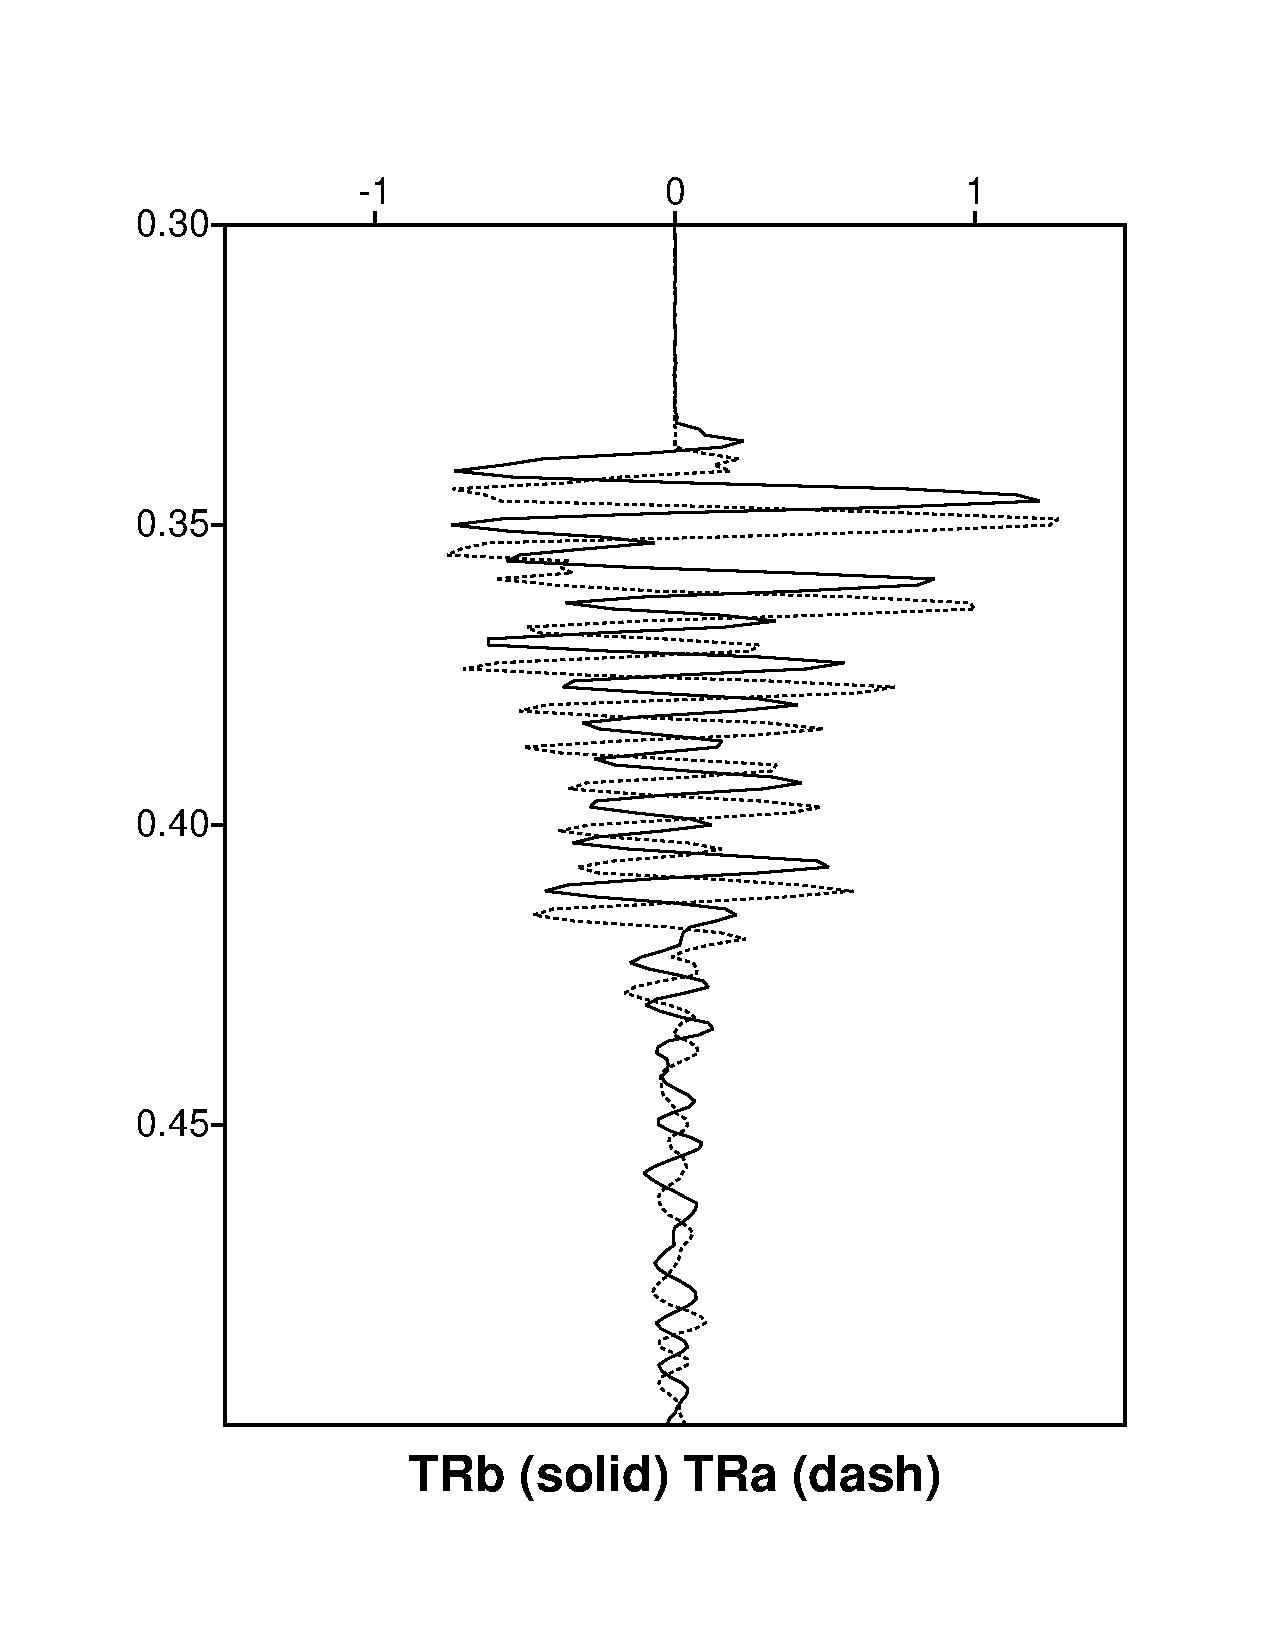
\includegraphics[width=0.45\textwidth]{Fig/fig1}
%    \label{fig:fig1}}\\
%    \subfloat[]{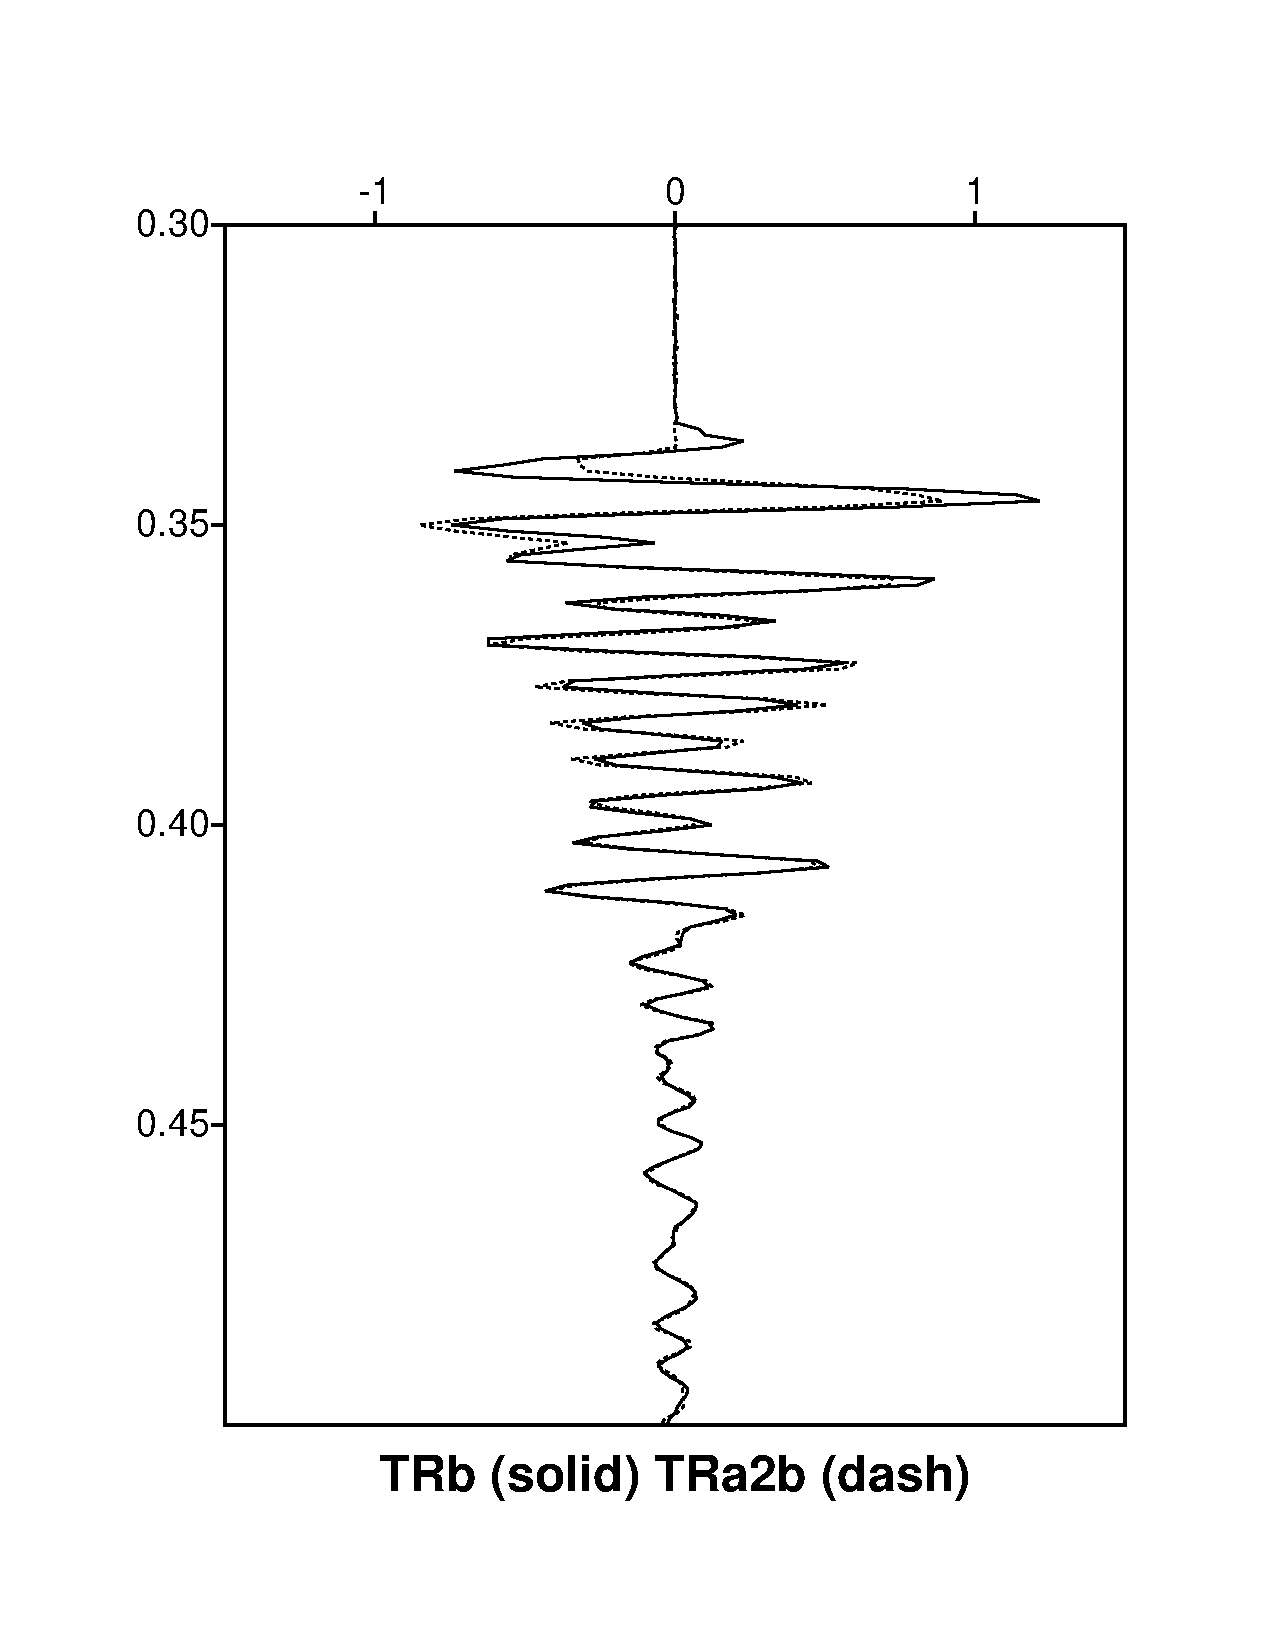
\includegraphics[width=0.45\textwidth]{Fig/fig2}
%    \label{fig:fig2}}\\
%	\caption{(a) Caption a. (b) Caption b.}
%	\label{fig:fig1,fig2}
%\end{figure}

%\begin{figure*}[ht!]
%	\centering
%	\subfloat[]{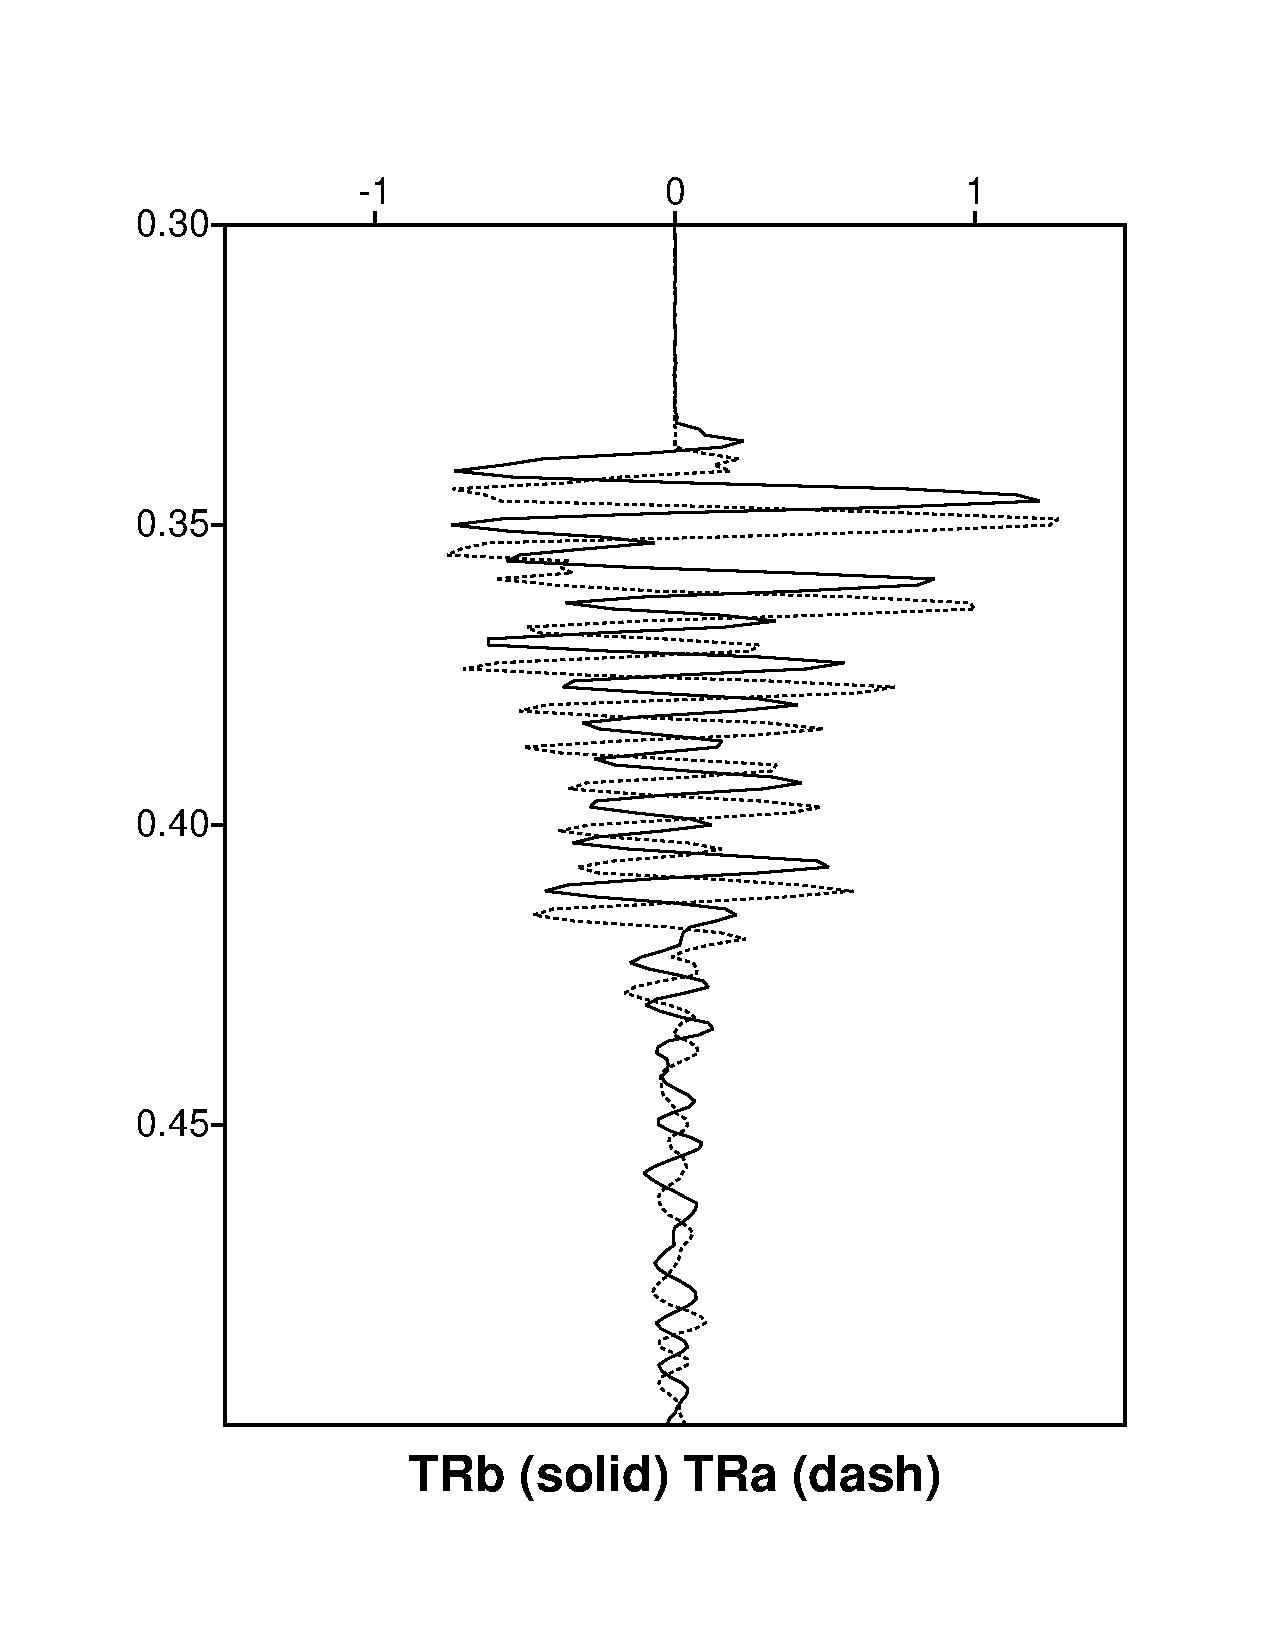
\includegraphics[width=0.45\textwidth]{Fig/fig1}
%    \label{fig:fig1}}\\
%    \subfloat[]{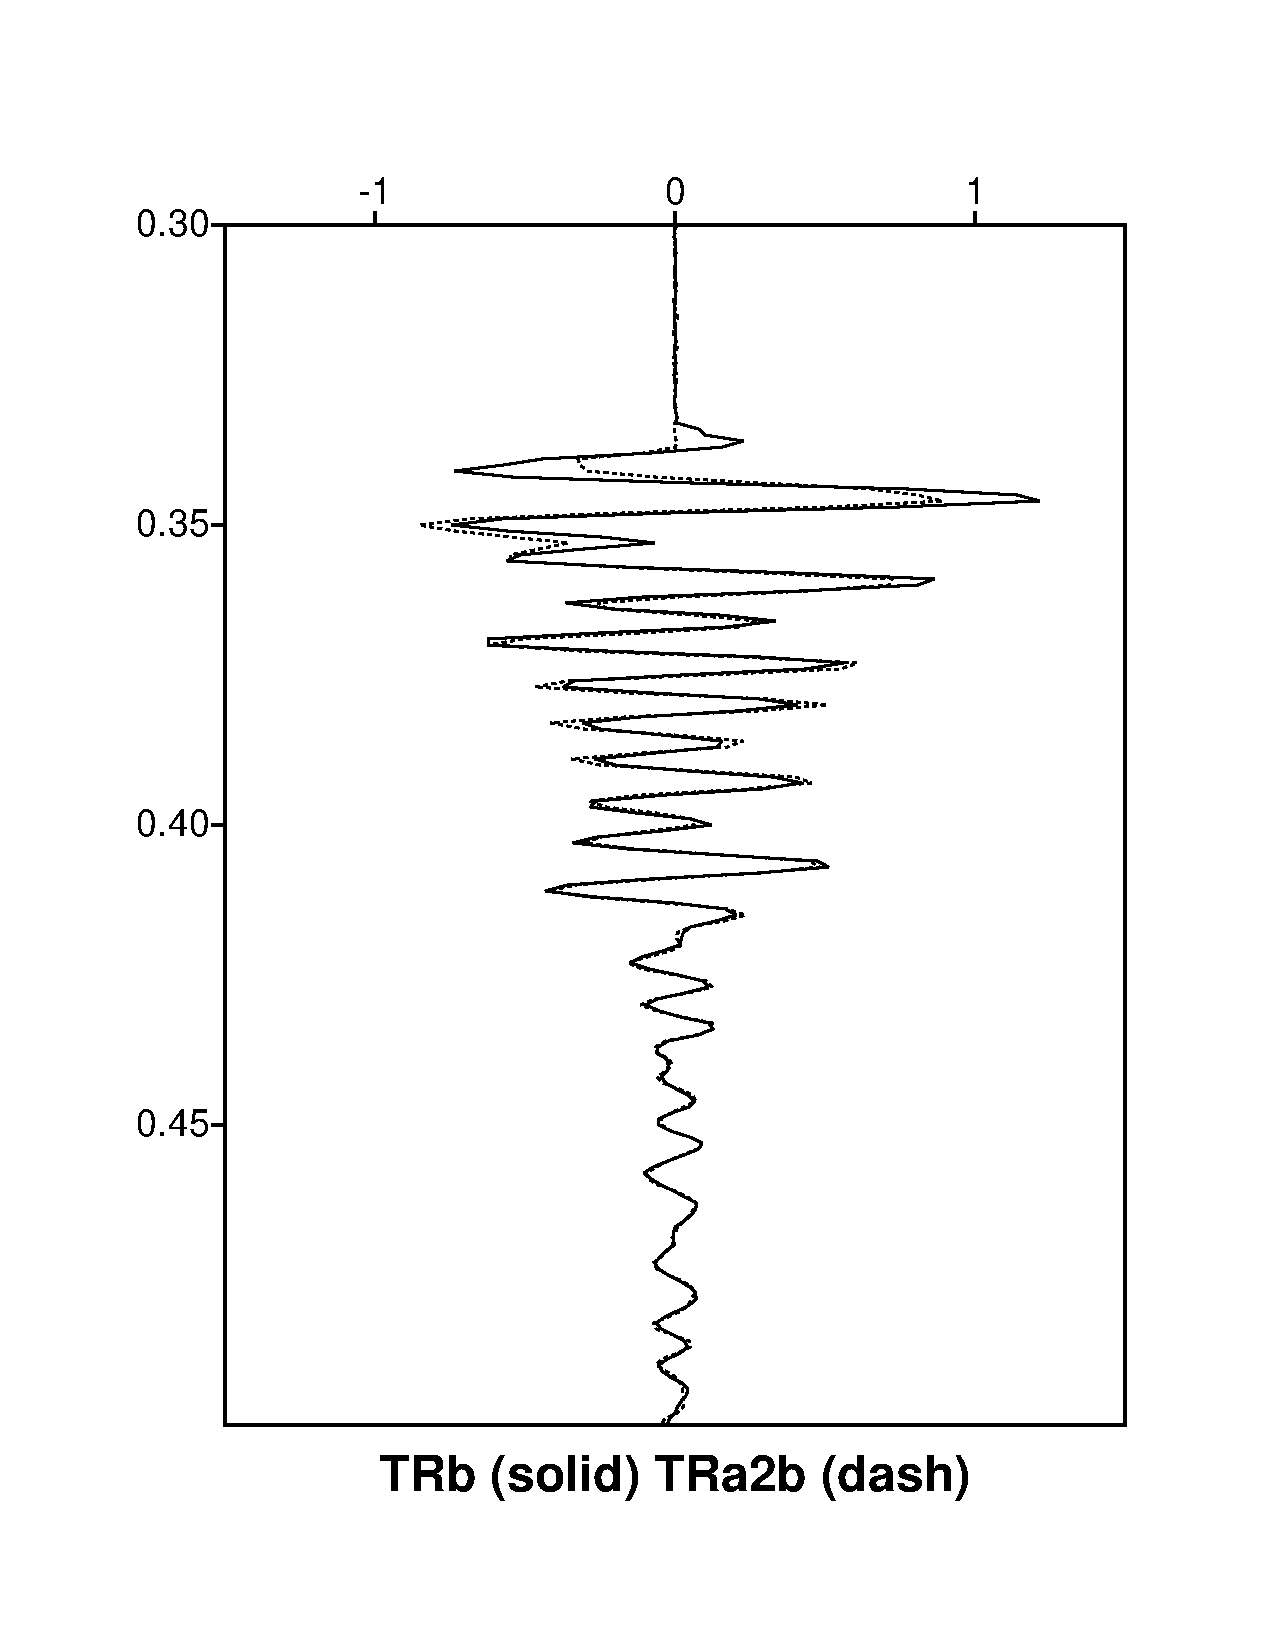
\includegraphics[width=0.45\textwidth]{Fig/fig2}
%    \label{fig:fig2}}\\
%	\caption{(a) Caption a. (b) Caption b.}
%	\label{fig:fig1,fig2}
%\end{figure*}

%\begin{table}[h]
%\caption{Table caption}
%\begin{center}
%     \begin{tabular}{|c|c|c|c|c|c|} 
%	  \hline Column1 (unit)  & Column2 (unit) & Column3 (unit) \\ 
%	  \hline 1 & 2  & 3 \\
%       \hline
%    \end{tabular} 
%\end{center}
%\label{tbl:table1}
%\end{table}

